\chapter{Evaluation and Simulation Experiments}\label{sec:exp}
TODO

\section{Best Covariance Function for Plume Modelling}\label{sec:bestkernel}
To obtain the best covariance function including its parameters to approximate 
a plume distribution these were evaluated using the test-set method. For each of 
the single source Gaussian (G-NF-SS-SV), the single source dispersion 
(D-NF-SS-SV), and the multiple source dispersion (D-NF-MS-SV), all without 
noise, 50 random instances were created. For each instance a set sampling 
locations was generated using the Metropolis-Hastings based technique described 
in Chapter~\ref{sec:mh}. Herein, every fifth Metropolis-Hastings sample was used 
in the final set and was used as mean of Gaussian with a standard deviation 
$\sigma = \SI{6}{\meter}$ to draw five more samples to include in the final set.  
The proposal distribution of the Metropolis-Hastings algorithm was also 
a Gaussian with standard deviation $\sigma = \SI{6}{\meter}$. In addition, 1000 
uniformly samples were added to the final set of samples. All samples outside of 
the scenario volume were dismissed. From all kept sample points 1000 were 
randomly selected for training and the rest was used as test set to determine 
the error.

Obtaining the training samples in this way should roughly mirror a good sampling 
with an UAV with many samples in the areas of high concentration and a few in 
the remaining areas. The advantage using this way of sampling is that it allows 
us to test different kernels independently on the exact behavior of the UAV and 
time consuming simulation of it.

The kernels tested were the squared exponential, the Mat\'ern kernel with $\nu 
= 5/2$, the Mat\'ern kernel with $\nu = 3/2$, and the exponential kernel. The 
length scales tested ranged from \SI{1}{\meter} to \SI{100}{\meter}. The process 
variance was fixed as $\sigma\ped{k}^2 = 1$. Note that this parameter has no 
effect on the predictive mean as long as the assumed noise variance 
$\sigma\ped{n}^2$ is zero.

The average of the fraction of the remaining error is plotted in 
Figure~\ref{fig:lengthscales} for the different kernels and error measures. The 
minimum is roughly the same for all kernels and lies around $\ell 
= \SI{5}{\meter}$.  However, the behavior differs considerably for non-optimal 
length scales.  The smoother (the more often the kernel is differentiable) the 
more the error increases for too large length scales.  Especially, for the 
squared exponential covariance function this increase is quite abrupt. Only for 
very large length scales it decreases again for the squared exponential kernel.

\begin{figure}
    \centering
    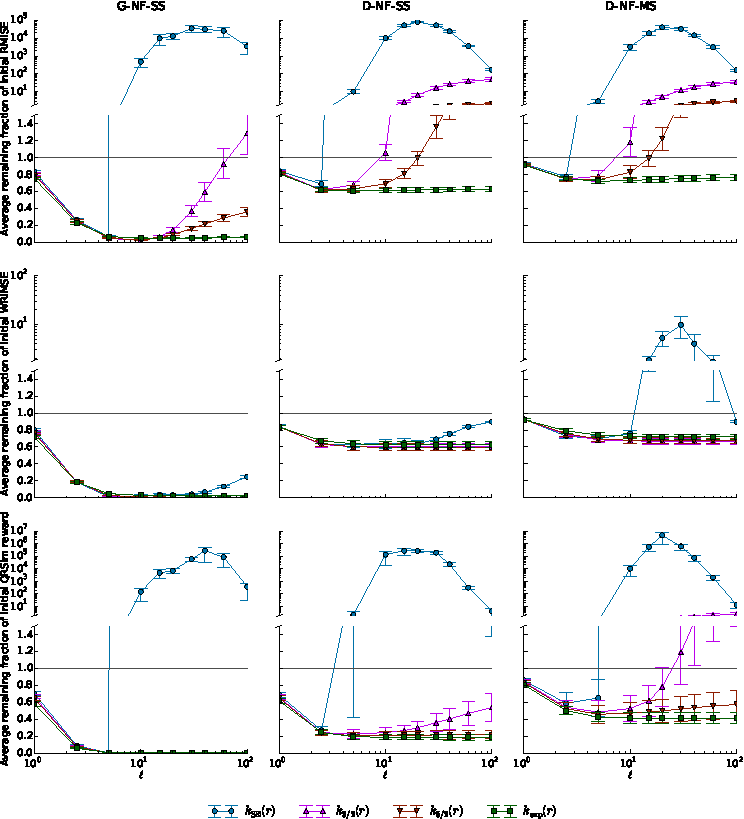
\includegraphics{plots/lengthscales}
    \caption[Influence of the length scale of the covariance functions]{The 
        average remaining fraction of the inital error for different covariance 
        function in dependence of length scale.  The rows correspond to the 
        RMISE, WRMISE, and QRSim reward error measures.  The columns correspond 
        to a single source Gaussian (G-NF-SS), a single source Gaussian 
        dispersion (D-NF-SS), and a multiple source Gaussian dispersion 
        (D-NF-MS). All scenarios were simulated without sensor noise.  Error 
        bars represent the standard error. The boundary of $1.0$ where the error 
        of the trained Gaussian process is larger than an all zero prediction is 
        marked with a horizontal line.}\label{fig:lengthscales}
\end{figure}

Comparing the WRMISE to the RMISE the former one stays quite low even for larger 
length scales. This indicates that in the area of the plume (also due to the more 
dense sampling) a good fit is still obtained, but around that area the 
prediction gets worse. Thus, the steep concentration gradients around the plume 
are not well captured in that case.

The results give also an idea how good of a fit can be expected at best when 
using an UAV\@. Whereas the fraction of the remaining error decreases to nearly 
zero for the single source Gaussian, it stays above 0.6 for the dispersion 
scenario with the more localized plume distribution. The reward error measure is 
decreased to lower levels, but this is likely to underestimation of the error at 
the plume boundaries as argued in Chapter~\ref{sec:qrsim-reward}.

Besides the error measures the log likelihood of each trained Gaussian process 
was calculated. In Figure~\ref{fig:loglikelihood} the average over trials is 
plotted. Only for the squared exponential kernel the maximum of the log 
likelihood corresponds to the minimum of the RMISE\@. Towards longer length 
scales the likelihood declines very steeply. Using the log likelihood to 
estimate the length scales for the other covariance functions would largely 
overestimate it.

\begin{figure}
    \centering
    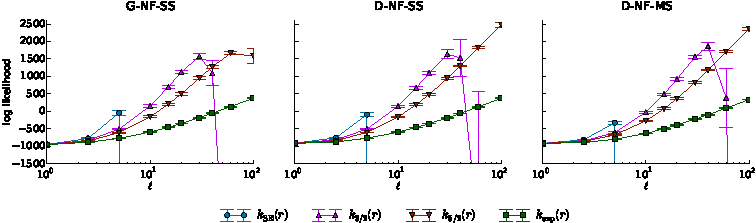
\includegraphics{plots/loglikelihood}
    \caption[Log likelihood in dependence of the kernel lengthscale]{The average 
        log likelihood of the training data in dependence of the length scale 
        using different kernels.  Each of the three plots shows one noise free 
        scenario of the single source Gaussian (G-NF-SS), single source Gaussian 
        dispersion (D-NF-SS), and multiple source Gaussian dispersion (D-NF-MS).  
        Error bars represent the standard error.}\label{fig:loglikelihood}
\end{figure}

Taken these results together it is best to choose a non-smooth kernel with 
a length scale of $\ell = \SI{5}{\meter}$. As it is advantageous to be able to 
use a gradient based optimizer for the optimization of acquisition functions, 
I decided to use the Matérn kernel with $\nu = 3/2$ in the further experiments, 
which gives a once mean square differentiable Gaussian process in opposite to 
the exponential kernel. Unfortunately, optimizing the length scale using the 
likelihood would not give good results and I fixed the length scale at $\ell 
= \SI{5}{\meter}$. Also, including a prior in the log likelihood does not help 
here. In example to shift the maximum of the likelihood for the chosen kernel to 
\SI{5}{\meter} a Gaussian prior would need a standard deviation of less then 
$\sigma_{\ell} < \e^{-2078} / \sqrt{2\uppi} \approx 0$ (see 
Apendix~\ref{sec:prior}).  Thus, effectively resulting in a fixed length scale.

\section{Comparison of Utility Functions}\label{sec:cmputility}
Given the kernel chosen in the previous section I continued to compare the 
different utility functions in the noiseless scenarios single source Gaussian 
(G-NF-SS-SV), single source dispersion (D-NF-SS-SV), and multiple source 
dispersion (D-NF-MS-SV).

For each given scenario 20~trials were performed. In each run the UAV first 
surrounded the simulation area in a height of \SI{40}{\meter} with a margin of 
\SI{10}{\meter} to the boundaries of the simulated volume. After that further 
way-points were chosen with one of the acquisition functions discussed in 
Chapter~\ref{sec:utility}. The optimization of that functions has been described 
in Chapter~\ref{sec:fnopt}.

Each trial was allowed to run for a maximum of \SI{3000}{\second} in simulation 
time. However, when a new target way-point was within \SI{3}{\meter} of the 
previous one the UAV was considered to become stuck in a maximum of the 
acquisition function and the simulation was stopped at that point to reduce 
overall simulation time. A plume measurement was taken every second.

The error measures were estimated as described in Chapter~\ref{sec:error}. The 
sampling locations for that where chosen as 1000 uniformly distributed sampling 
locations, every tenth of 4200 locations from the Metropolis-Hastings algorithm 
with Gaussian proposal distribution with standard deviation $\sigma 
= \SI{10}{\meter}$, and 10 more locations sampled from the proposal distribution 
for each of included Metropolis-Hastings samples.

I tested all three utility functions proposed in Chapter~\ref{sec:utility}: 
DUCB, PDUCB (with $\varepsilon = 10^{-30}$), and GO\@. DUCB was tested with 
a constant scaling factor of $s\ped{DUCB}(\vc y) = 1$ and the automatic scaling 
in Equation~\ref{eqn:scale-ducb}.  PDUCB was tested with a constant scaling 
factor of $s\ped{PDUCB}(\vc y) = 70$ (a little bit more than $-\log 
\varepsilon$) and the automatic scaling in Equation~\ref{eqn:scale-pducb}.  
Furthermore, I performed a parameter search over $\kappa \in \cbr{0.1, 0.5, 
0.75, 1, 1.25, 1.5, 2}$ and $\gamma \in \cbr{0} \cup \cbr{-10^p | p = -9, -8, 
  \dots, -2}$. Note that for the GO utility function the $\kappa$ parameter has 
no effect.

Figure~\ref{fig:psearch-G-NF-SS-SV}--\ref{fig:psearch-D-NF-MS-SV} visualize the 
average remaining fraction of the error for the different scenarios.  The 
respective parameters and values of the minima are listed in Table~TODO\@.  The 
average reduction (over trials) of the RMISE against simulation time in the 
single source Gaussian scenario (G-NF-SS-SV) is plotted in 
Figure~\ref{fig:errtrace-nf} and looks essentially the same for WRMISE and the 
QRSim reward and therefore it is not shown fer those measures.

\begin{figure}
    \centering
    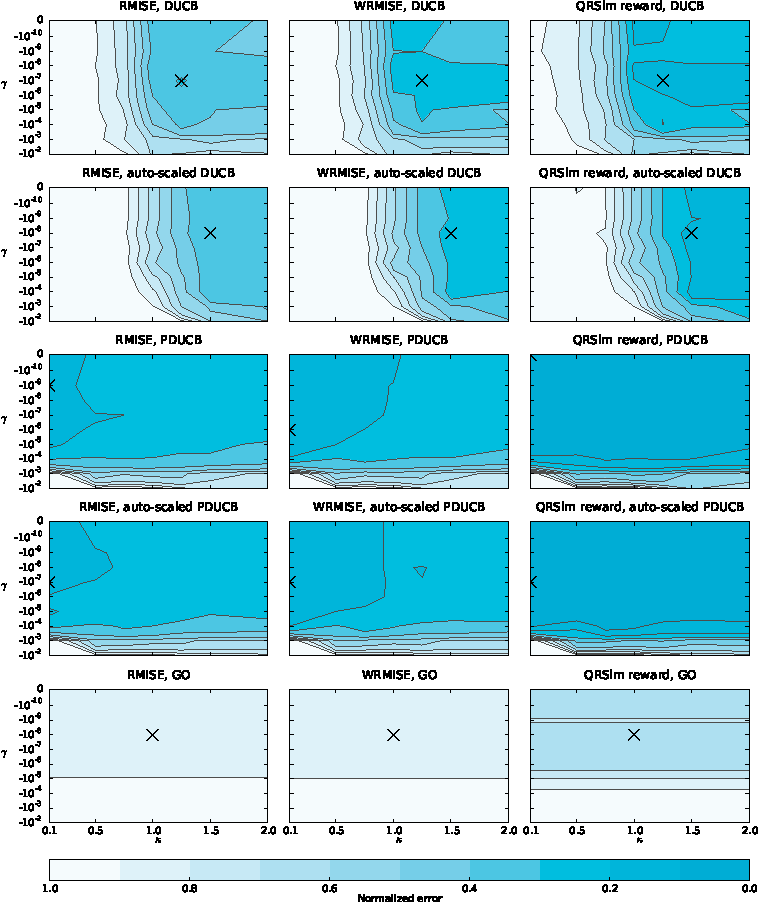
\includegraphics{plots/psearch-G-NF-SS-SV}
    \caption[Remaining fraction of the initial error (G-NF-SS-SV)]{The average 
        remaining fraction of the initial error for different measures, utility 
        functions, parameters in the noiseless single source Gaussian scenario 
        (G-NF-SS-SV).  The columns represent the RMISE, WRMISE, and QRSim reward 
        error measure.  The rows represent the DUCB, auto-scaled DUCB, PDUCB, 
        auto-scaled PDUCB and GO utility functions. The auto-scaled versions use 
        the scaling factor defined in Equations~\ref{eqn:scale-ducb} 
        and~\ref{eqn:scale-pducb}, in contrast to a constant scaling factor. The 
        minimum of each plot is marked with 
        cross.}\label{fig:psearch-G-NF-SS-SV}
\end{figure}
\begin{figure}
    \centering
    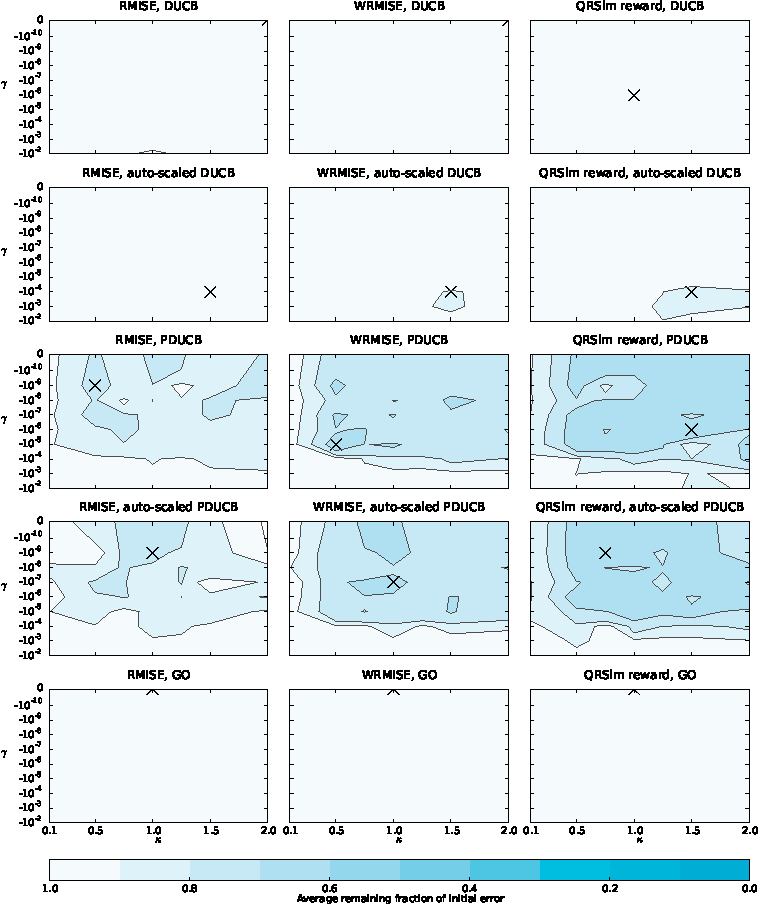
\includegraphics{plots/psearch-D-NF-SS-SV}
    \caption[Remaining fraction of the initial error (D-NF-SS-SV)]{The average 
        remaining fraction of the initial error for different measures, utility 
        functions, parameters in the noiseless single source Gaussian dispersion 
        scenario (D-NF-SS-SV).  The columns represent the RMISE, WRMISE, and 
        QRSim reward error measure.  The rows represent the DUCB, auto-scaled 
        DUCB, PDUCB, auto-scaled PDUCB and GO utility functions. The auto-scaled 
        versions use the scaling factor defined in 
        Equations~\ref{eqn:scale-ducb} and~\ref{eqn:scale-pducb}, in contrast to 
        a constant scaling factor.  The minimum of each plot is marked with 
        cross.}\label{fig:psearch-D-NF-SS-SV}
\end{figure}
\begin{figure}
    \centering
    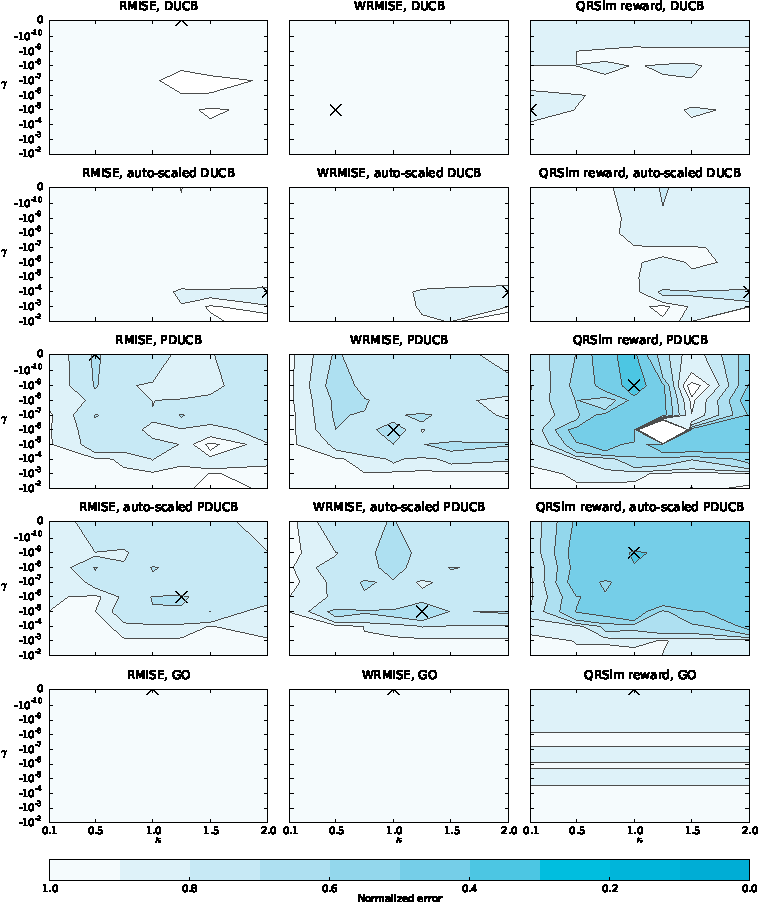
\includegraphics{plots/psearch-D-NF-MS-SV}
    \caption[Remaining fraction of the initial error (D-NF-MS-SV)]{The average 
        remaining fraction of the initial error for different measures, utility 
        functions, parameters in the noiseless multiple source Gaussian 
        dispersion scenario (D-NF-SS-SV).  The columns represent the RMISE, 
        WRMISE, and QRSim reward error measure.  The rows represent the DUCB, 
        auto-scaled DUCB, PDUCB, auto-scaled PDUCB and GO utility functions. The 
        auto-scaled versions use the scaling factor defined in 
        Equations~\ref{eqn:scale-ducb} and~\ref{eqn:scale-pducb}, in contrast to 
        a constant scaling factor.  The minimum of each plot is marked with 
        cross.}\label{fig:psearch-D-NF-MS-SV}
\end{figure}
\begin{figure}
    \centering
    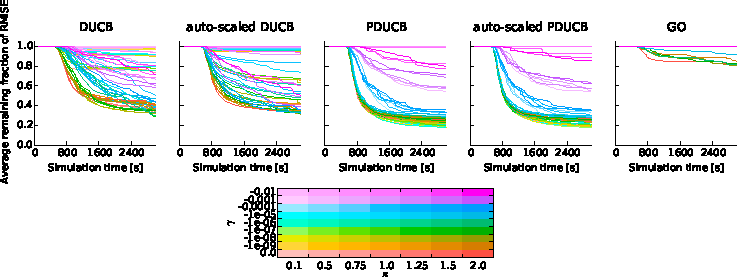
\includegraphics{plots/errtrace-nf}
    \caption[Time-course of the error reduction]{The average remaining fraction 
        of the initial RMISE in the single source Gaussian scenario 
        (G-NF-SS-SV).  Each individual plot corresponds to one utility function 
        and scaling.  The auto-scaled versions use the scaling factor defined in 
        Equations~\ref{eqn:scale-ducb} and~\ref{eqn:scale-pducb}, in contrast to 
        a constant scaling factor. The $\gamma$ parameter is coded by hue and 
        the $\kappa$ parameter by lightness.}\label{fig:errtrace-nf}
\end{figure}

This is a rich dataset from which quite a few insights can be gained. First of 
all it can be noted that the GO acquisition function does not perform very well.  
Even in the single source Gaussian scenario the RMISE is only reduced by about 
\SI{20}{\percent} and in the other two scenarios it performs even worse.

Comparing DUCB and PDUCB the latter one consistently performs better with 
a reduction in the RMISE and WRMISE by about additional \SI{15}{\percent} or 
more. Also, PDUCB has a lower standard deviation in the single source Gaussian 
scenario. Despite that, its standard deviation is higher than that of DUCB in 
the dispersion scenarios.

In the single source Gaussian scenario PDUCB proves to be quite robust against 
the choice of $\kappa$ as for all values very good results are obtained. This 
picture is a bit more noisy in the dispersion scenarios. It seems that too low 
values ($\kappa < 0.75$) degrade performance. This is consistent with the 
argument in Chapter~\ref{sec:utility} that too low $\kappa$ limit the 
exploration and let the UAV become stuck in a (local) maximum. The choice of 
$\gamma$ has no considerable effect as long as the distance penalty is not 
chosen too large ($\gamma < -10^{-5}$).

The same behavior for the choice of $\gamma$ is also observed for DUCB in the 
single source Gaussian scenario. However, this utility function is far more 
sensitive to the choice of $\kappa$. Using the scaling $s\ped{DUCB}(\vc y) = 1$ 
the performance degrades setting $\kappa < 1$ and using the automatic scaling it 
degrades for $\kappa < 1.5$. In the dispersion scenarios the DUCB acquisition 
function does not perform well for any tested combination of parameter values.

Interestingly,  DUCB performs slightly better with the automatic scaling, 
whereas PDUCB performs slightly worse.

Finally, taking a look at the time course of error reduction multiple phases can 
be discovered where a reasonable reduction of the error occurs. About the first 
\SI{500}{\second} nearly no reduction occurs as in this phase the UAV only 
surround the area of interest. Then the error rapidly decreases in the next 
\SIrange{1000}{2000}{\second} until the decrease levels off and stays fairly 
constant for the rest of the simulation time.

These results show that PDUCB outperforms the DUCB and GO acquisition functions 
and in addition is quite robust against a non-optimal choice of parameters. The 
especially bad performance of the GO utility function is not too surprising at 
its intended use is to find a function maximum and not building a correct model 
of the function (respectively plume concentration).  DUCB works reasonable well 
for the simple case of a Gaussian distribution, but fails for the more localized 
dispersions.

The PDUCB performance might not seem to be too impressive in the dispersion 
scenarios, too. However, one has to keep in mind that even in 
Section~\ref{sec:bestkernel} with much more samples the error could not be 
reduced to less than TODO\SI{1}{\percent}.  Also, the qualitatively the plume is 
predicted at the correct location as Figure~TODO shows, despite some deviance of 
the exact concentration values.

Given this discussion I selected the PDUCB acquisition function with automatic 
scaling, $\kappa = 1.25$, and $\gamma = -10^{-8}$ for further experiments.  
Though the automatic scaling performs a little bit worse, I consider it to be 
advantageous as it decouples the other parameter values from the exact 
concentration levels of the plume dispersion.

TODO explain kappa and gamma
TODO example run visualizations

\section{Noisy}

\section{Multiple UAVs}

